\chapter{Harmonogram Realizacji Projektu}
\label{chap:harmonogram}
Prace rozpoczęto od faza analizy i planowania, która zajęła pierwszy dzień. Drugiego dnia zrealizowano projekt bazy danych. Najdłuższy, trwający od trzeciego do piątego dnia, był etap implementacji kluczowych modułów systemu. Szósty dzień w całości poświęcono na testowanie funkcjonalności i wprowadzanie niezbędnych poprawek. Ostatni, siódmy dzień, przeznaczono na przygotowanie kompletnej dokumentacji technicznej i użytkowej projektu (Rys. \ref{fig:harmonogram_gantta}).

\begin{figure}[H]
    \centering
    \includegraphics[width=\textwidth]{figures/harmonogram_gantta.png}
    \caption{Diagram Gantta przedstawiający tygodniowy harmonogram prac nad projektem.}
    \label{fig:harmonogram_gantta}
\end{figure}

\chapter{Prezentacja Warstwy Użytkowej Projektu}
\label{sec:logowanie}

Pierwszym elementem, z którym użytkownik ma styczność, jest okno logowania. Zostało ono zaprojektowane w celu weryfikacji tożsamości użytkownika i nadania mu odpowiednich uprawnień w systemie. Interfejs okna logowania (Rys. \ref{fig:logowanie}) składa się z pól tekstowych do wprowadzenia nazwy użytkownika i hasła oraz przycisku "Zaloguj". Pola te są obsługiwane przez komponenty `JTextField` dla loginu i `JPasswordField` dla hasła, co zapewnia maskowanie wpisywanych znaków.

\begin{figure}[H]
	\centering
	\includegraphics[width=0.8\textwidth]{figures/Logowanie.png}
	\caption{Główne okno logowania do systemu.}
	\label{fig:logowanie}
\end{figure}

Po kliknięciu przycisku "Zaloguj", uruchamiany jest `ActionListener`. Proces weryfikacji przebiega następująco:
\begin{enumerate}
	\item Pobierane są dane z pól `LoginInput` i `PasswordInput`.
	\item Następuje walidacja, czy pola nie są puste. Jeśli tak, wyświetlany jest komunikat z prośbą o uzupełnienie danych.
	\item Konstruowane jest zapytanie SQL, które ma na celu odnalezienie użytkownika o podanym loginie i haśle w bazie danych. Zapytanie łączy tabele `uzytkownicy` i `strazacy`, aby pobrać rolę, imię oraz nazwisko strażaka.
	\item Na podstawie pobranej z bazy roli, system decyduje, które okno aplikacji otworzyć – `Start` dla administratora lub `UzytkownikStart` dla zwykłego użytkownika.
	\item W przypadku błędnych danych, użytkownik widzi stosowny komunikat (Rys. \ref{fig:logowanie_blad}). System jest również przygotowany na obsługę błędów połączenia z bazą danych.
\end{enumerate}

\begin{figure}[H]
	\centering
	\begin{subfigure}{0.48\textwidth}
		\centering
		\includegraphics[width=\linewidth]{figures/UdaneLogowanie.png}
		\caption{Komunikat o pomyślnym zalogowaniu.}
		\label{fig:logowanie_sukces}
	\end{subfigure}
	\hfill
	\begin{subfigure}{0.48\textwidth}
		\centering
		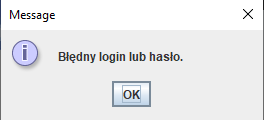
\includegraphics[width=\linewidth]{figures/BladLogowania.png}
		\caption{Komunikat o błędnych danych logowania.}
		\label{fig:logowanie_blad}
	\end{subfigure}
	\caption{Komunikaty zwrotne w procesie logowania.}
	\label{fig:komunikaty_logowania}
\end{figure}

\section{Główne Menu Aplikacji}
\label{sec:glowne_menu}

Po pomyślnym zalogowaniu użytkownik zostaje przekierowany do głównego menu, które stanowi centralny punkt nawigacyjny aplikacji. Interfejs menu (Rys. \ref{fig:menu}) zawiera przyciski nawigacyjne: "Strażacy", "Interwencje", "Pojazdy" oraz przycisk "Wyloguj". Każdy z przycisków posiada zaimplementowany `ActionListener`, który po kliknięciu zamyka aktualne okno (`dispose()`) i otwiera nowe, odpowiadające wybranej funkcjonalności. Na przykład, kliknięcie "Strażacy" tworzy i wyświetla obiekt klasy `Strazacy`.

\begin{figure}[H]
	\centering
	\includegraphics[width=0.8\textwidth]{figures/GlowneMenu.png}
	\caption{Główne menu aplikacji.}
	\label{fig:menu}
\end{figure}

